\section{Model Dynamics}

The dynamics, that emerge from this model, are very similar to the dynamics of the original model described in \Cref{sec:og.dynamics}.
\Cref{fig:final.period.whole.full} shows a 2D scan showing the periods of the stable cycles in the model.
This looks similar to \Cref{fig:yunus.2pi.2d.full}, which is the corresponding 2D scan of the original model.
\Cref{fig:final.period.whole.halved} shows a 2D scan of the halved model, similar to the 2D scans of the halved original model \Cref{fig:yunus.pi.2d.full}.
The reason for scanning the halved model is that we can detect ``type B'' parameter regions this way.
This approach is thoroughly described in \Cref{sec:og.halved}.

\begin{figure}
    \centering
    \begin{subfigure}{0.4\textwidth}
        \centering
        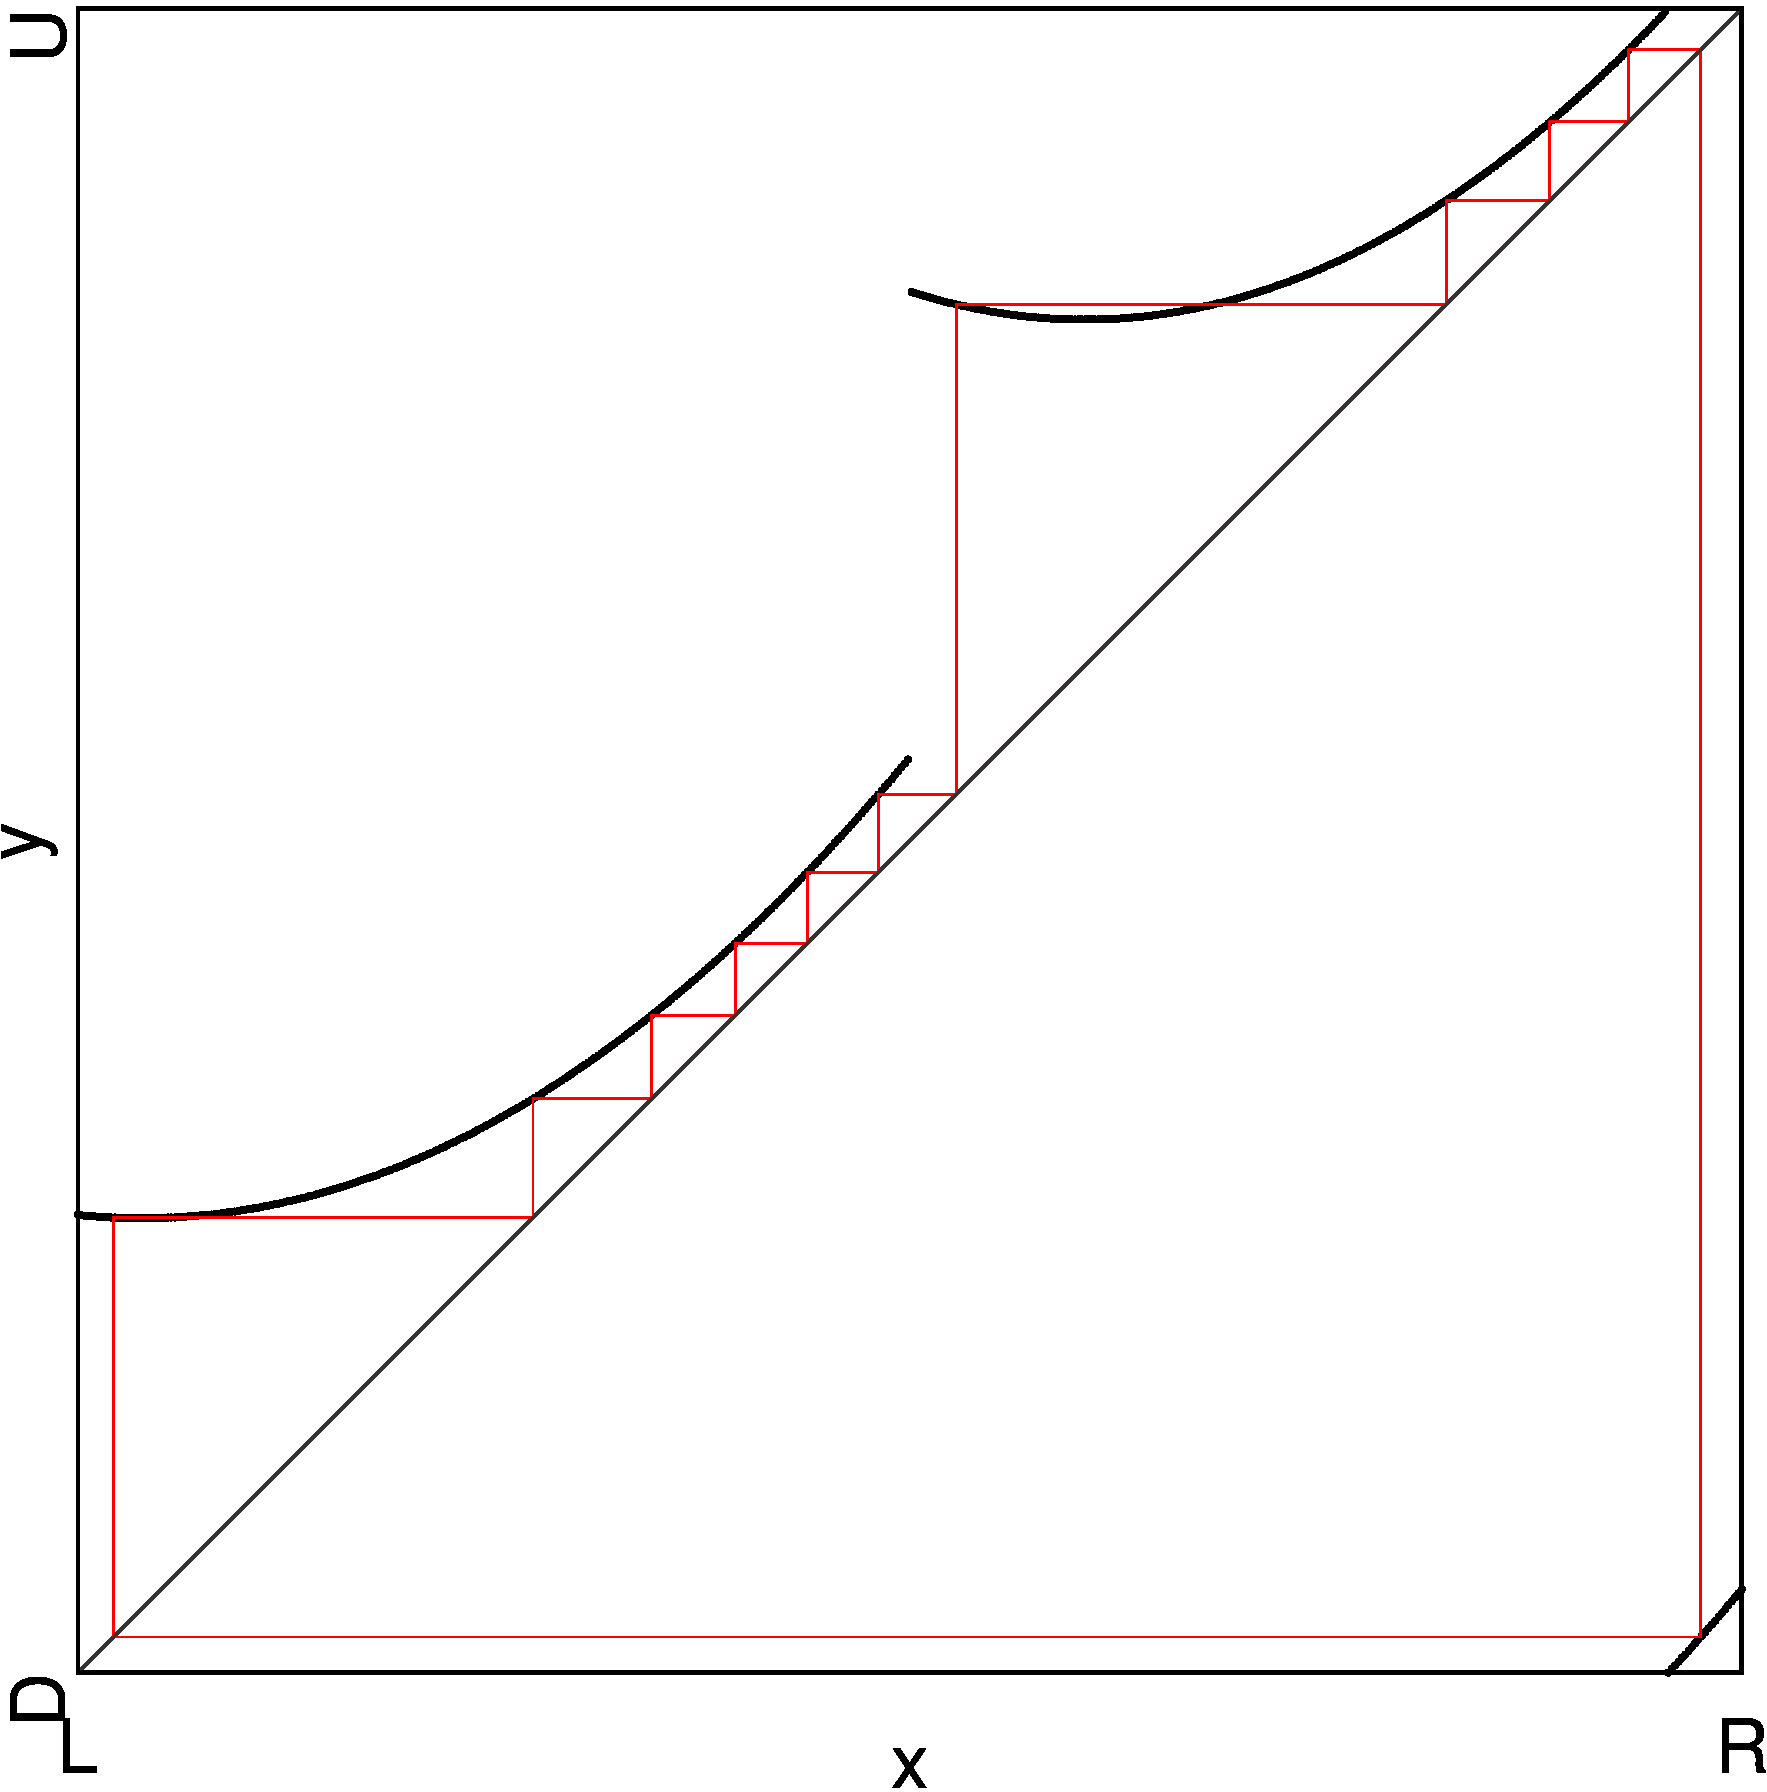
\includegraphics[width=\textwidth]{60_Final/2D_Period_Whole_Lotta_Points/result.png}
        \caption{Full Model}
        \label{fig:final.period.whole.full}
    \end{subfigure}
    \begin{subfigure}{0.4\textwidth}
        \centering
        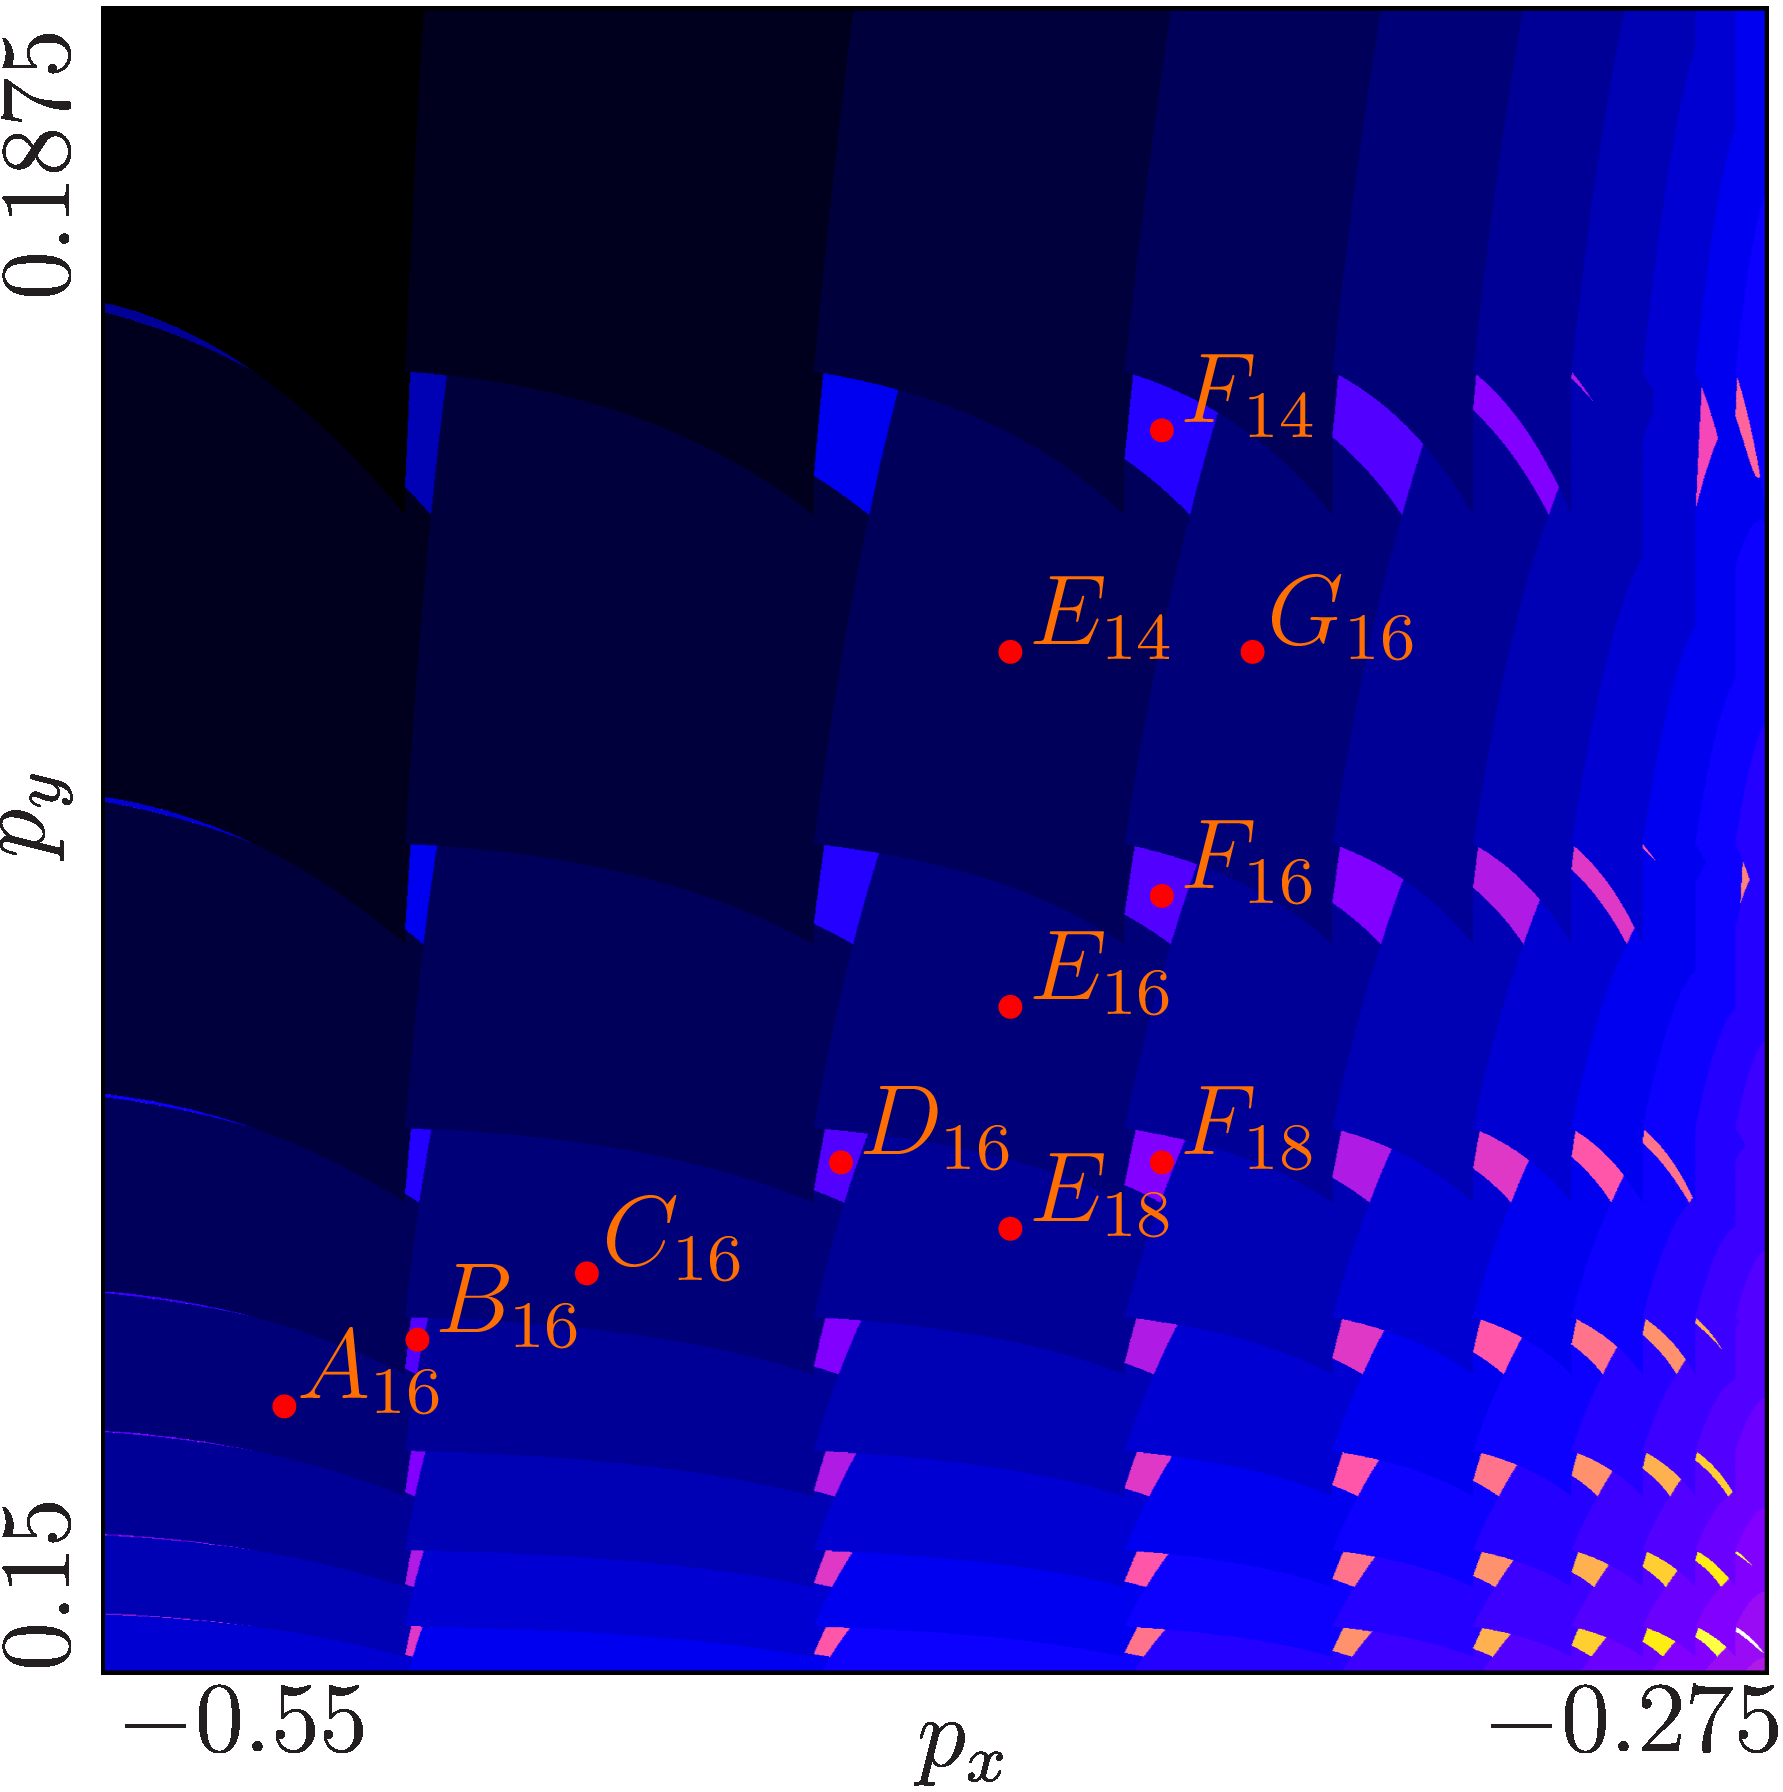
\includegraphics[width=\textwidth]{60_Final/2D_Period_Whole_Lotta_Points/result-halved.png}
        \caption{Halved Model}
        \label{fig:final.period.whole.halved}
    \end{subfigure}
    \caption{2D Scans of Periods of Final Model}
\end{figure}


